\section{Introduction}
\comment{
\begin{frame}{}
	\begin{itemize}
		\item A little bit of history
		\item Different flavours of AI 
		\item Machine learning
		\begin{itemize}
			\item[-] Description, types 
			\item[-]A little bit of math 
			\item[-] An illustrative example
		\end{itemize}
		\item If time permits 
		\begin{itemize}
			\item[-] ImageNet challenges and Deep neural networks 
			\item[-] Convolution networks, auto-encoders, transfer learning
			\item[-] Adversarial networks 
			\item[-] Other architectures 
		\end{itemize}
	\end{itemize}
\end{frame}
}

\begin{frame}{Imitation game}
		\begin{columns}
			\begin{column}{.5\textwidth}
				\begin{figure}
					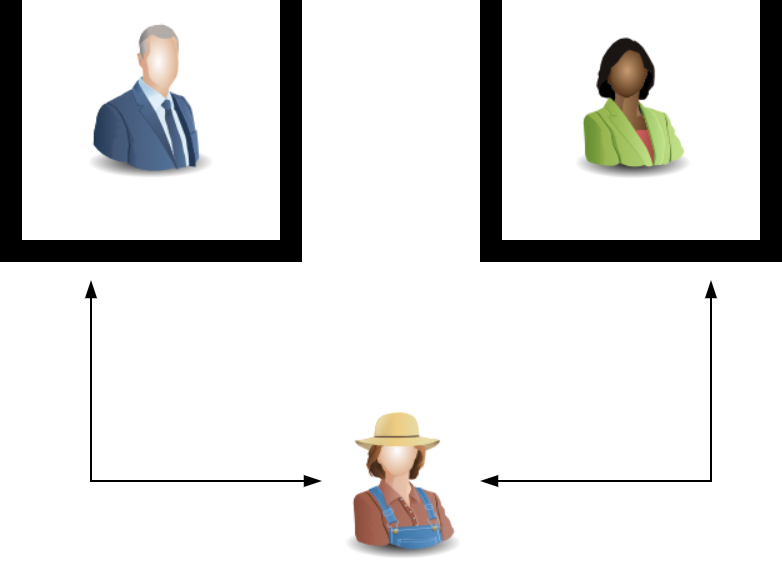
\includegraphics[width=.75\textwidth, center]{figures/imitation_game_1}
					\caption*{Interrogator}
				\end{figure}
			\end{column}
			\begin{column}{.5\textwidth}
				\begin{figure}
					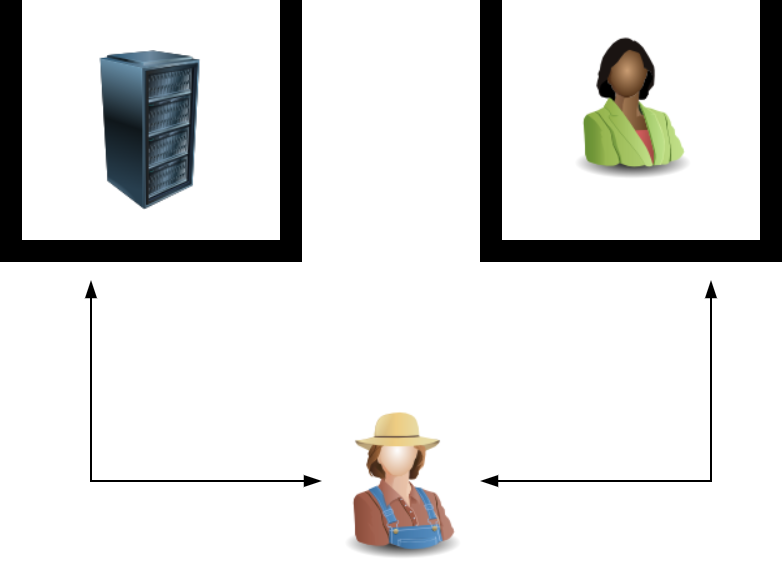
\includegraphics[width=.75\textwidth, center]{figures/imitation_game_2}
					\caption*{Interrogator}
				\end{figure}				
			\end{column}
		\end{columns}
\end{frame}


\begin{frame}{Artificial intelligence}
	\begin{itemize}
		\item Logic machines (50s)
		\item Knowledge based expert systems (80s)
		\item Language translation (60s) , 2000s, 2014 and later.  
		\item Machine learning 
			\begin{itemize}
				\item Neural networks including deep learning (started in 1943)
				\item Support vector machines 
				\item Baysian learning   
			\end{itemize}
		\item Graphs
		\item Genetic algorithms and genetic programs.
	\end{itemize}
\end{frame}


\begin{frame}{Expert systems}
		\begin{itemize}
			\item Database of formally described "facts" or "knowledge". 
			\item A reasoning engine for answering questions or solving problems.  
		\end{itemize}
	Not to be confused with a true natural language processing and 
	question-answering system. 
\end{frame}

\begin{frame}{Search}
	\begin{columns}
		\begin{column}{.5\textwidth}
			\begin{figure}
				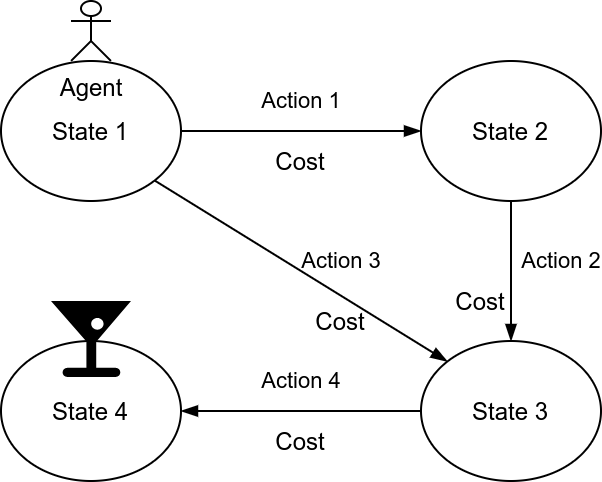
\includegraphics[width=.9\textwidth, center]{figures/ai_search_simple}
				\caption*{?}
			\end{figure}
		\end{column}
		\begin{column}{.5\textwidth}
			\begin{figure}
				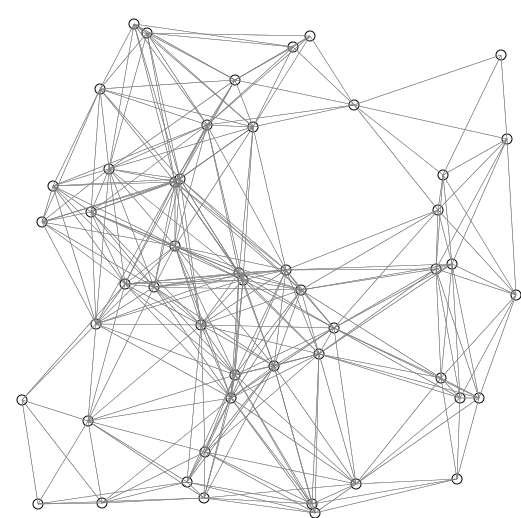
\includegraphics[width=.75\textwidth, center]{figures/DijkstraDemo-0}
				\caption*{?}
			\end{figure}
		\end{column}
	\end{columns}
\end{frame}

\begin{frame}{Neural Networks}
	
	{\scriptsize 
	\begin{description}
		\item[1943:] Warren McCulloch and Walter Pits connected neurons, computation, logic and learning.
		\item[1950:] Minsky and Dean Edmonds build first neural network computer. 3000 vacuum tubes, surplus 
		auto-pilot parts from B-24 bomber. 40 Neurons. 
		\item[1969:] Minsky and Papert publishobama-funny perceptron - simple linear networks could not learn basic 
		functions. 
		\item[1980s:] David Rumelhart, Jeff Hinton and Ronald Williams applied back propagation 
		(again) for training multi-layer neural networks. Rumelhart's work also created the foundations for 
		Recurrent Neural Networks. 
		\item[1990s:] LSTM networks by Hochreiter and Schmidhuber 1997. CNN for handwritten digit recognition - Yann LeCun. 
		\item[2000s:] LSTMs show promise in speech recognition 
		\item[2012:] Deep learning
	\end{description}
	}
\end{frame}

\begin{frame}{Different views}
	\begin{columns}
		\begin{column}{.5\textwidth}
			\begin{figure}
				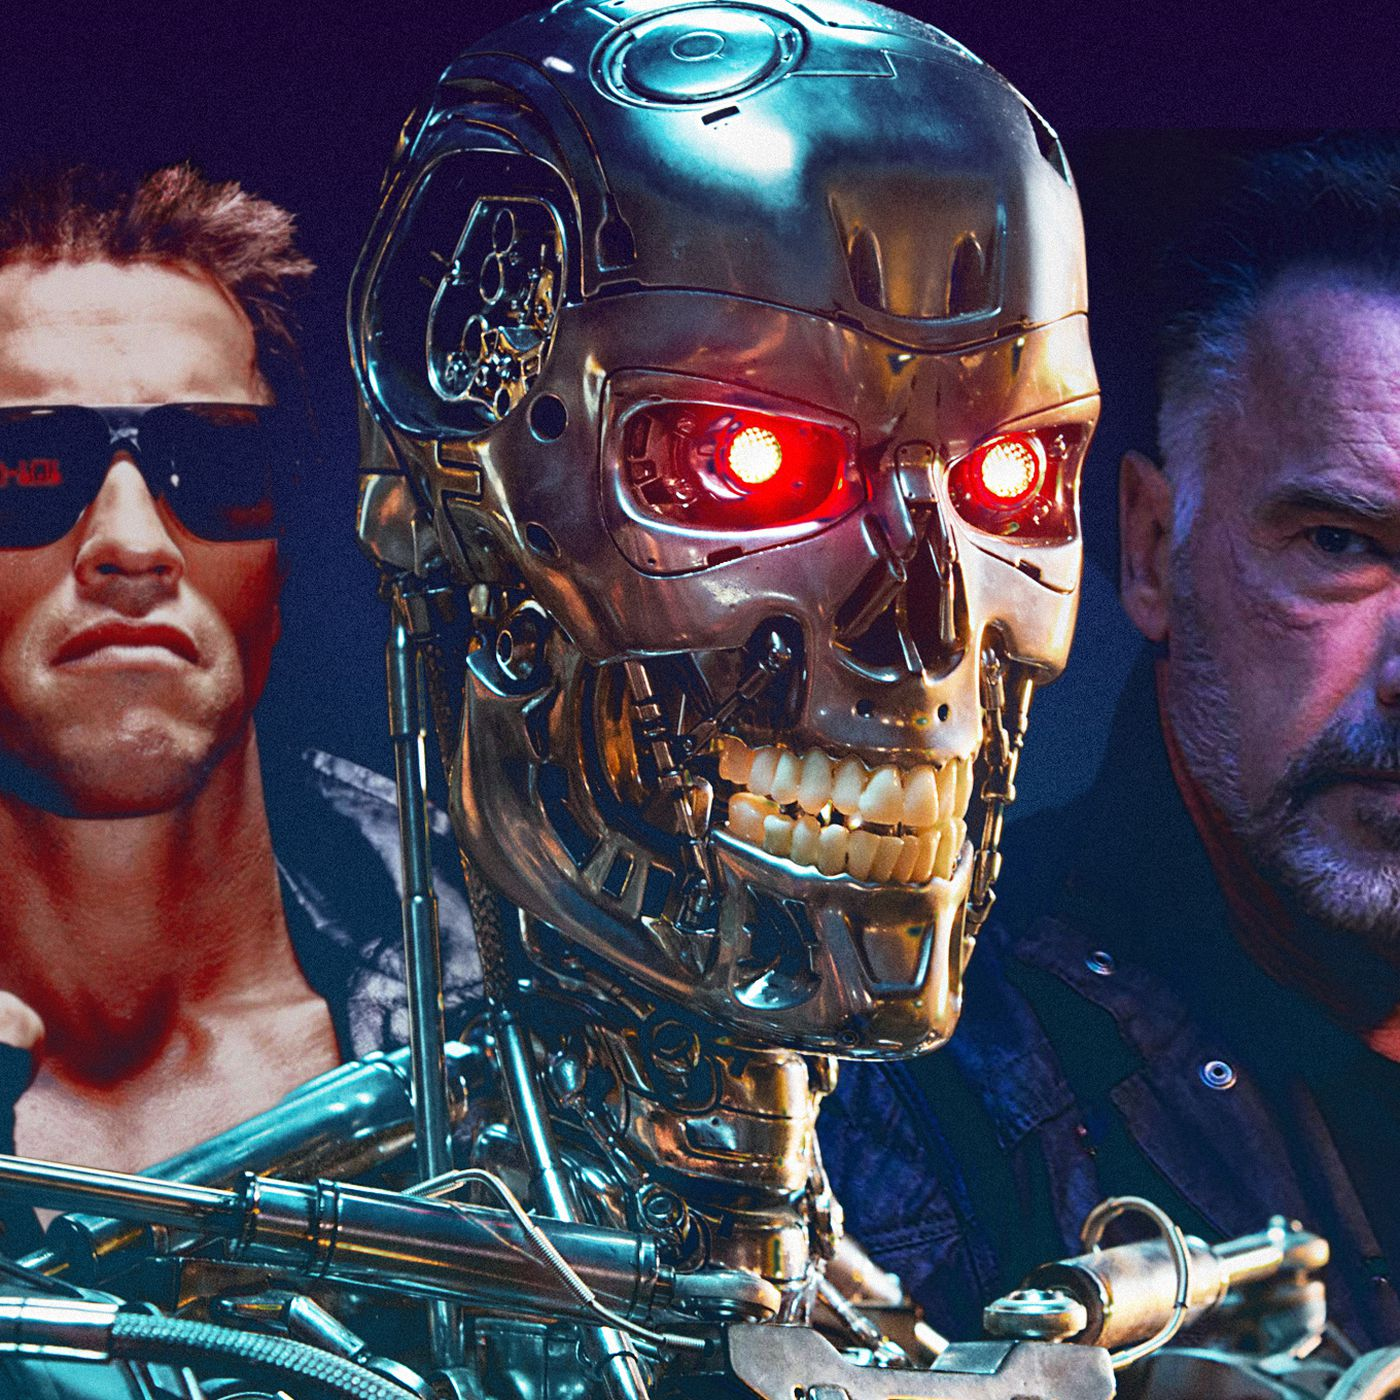
\includegraphics[width=.75\textwidth, center]{figures/terminator_001}
				\caption*{Agent}
			\end{figure}
		\end{column}
		\begin{column}{.5\textwidth}
			
			\begin{figure}
				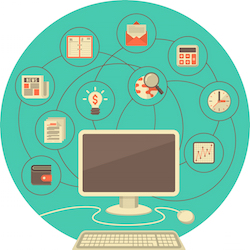
\includegraphics[width=.75\textwidth, center]{figures/WHU-lesson-6}
				\caption*{Tool}
			\end{figure}
		\end{column}
	\end{columns}
	\begin{columns}
		\begin{column}{.5\textwidth}
			\begin{center}
				General
			\end{center}
		\end{column}
		\begin{column}{.5\textwidth}
			\begin{center}
			\href{https://www.youtube.com/watch_popup?v=vIci3C4JkL0}{Narrow}	
			\end{center}
		\end{column}
	\end{columns}
\end{frame}




